% ============================================================
% Section 5.3: Wheelchair Navigation and Safety System Results
% ============================================================
\section{Wheelchair Navigation and Safety System Results}
\label{sec:wheelchair_navigation_safety_results}

The performance of the mobility subsystem and its integrated autonomous safety layer was evaluated under real-time navigational conditions. The operational objective was to quantify the latency of motor actuation in response to voluntary blink commands (forward, reverse, rotation, and stop) and to validate the efficacy of the obstacle avoidance mechanisms in dynamic environments.

\FloatBarrier
\subsection{Motor Actuation and Command Responsiveness}
\label{subsec:motor_actuation_responsiveness}

Following the extraction and classification of EOG blink sequences by the central processing unit, navigational commands were transmitted wirelessly to the embedded microcontroller (Arduino) via Bluetooth. The system demonstrated highly responsive physical actuation across all directional states. The L298N motor driver executed smooth transitions during acceleration and deceleration phases, which is critically important for minimizing mechanical jerks and ensuring the physical stability of patients with severe neuromuscular deficits. The delay between command reception and physical wheel rotation was negligible, enabling fluid, real-time trajectory adjustments.

\FloatBarrier
\subsection{Autonomous Obstacle Avoidance and Safety Override}
\label{subsec:autonomous_obstacle_avoidance}

A primary engineering challenge in bio-guided mobility is protecting the user from collisions resulting from delayed or erroneous physiological inputs. To address this, an independent environmental monitoring layer was embedded directly into the Arduino firmware.

The ultrasonic Time-of-Flight (ToF) sensor array was calibrated with strict proximity thresholds: a $40\,\text{cm}$ safety perimeter for the front sensor and a $30\,\text{cm}$ perimeter for the rear sensor. Experimental testing confirmed the high efficiency of the embedded code; whenever an obstacle breached these predefined perimeters, the microcontroller instantly executed a hardware-level interrupt. This safety protocol successfully overrode any active EOG user commands, immediately arresting motor operation to prevent collision without requiring intervention from the MATLAB processing layer. Figure~\ref{fig:ultrasonic_tof_results} illustrates this proximity threshold monitoring.

\begin{figure}[H]
  \centering
  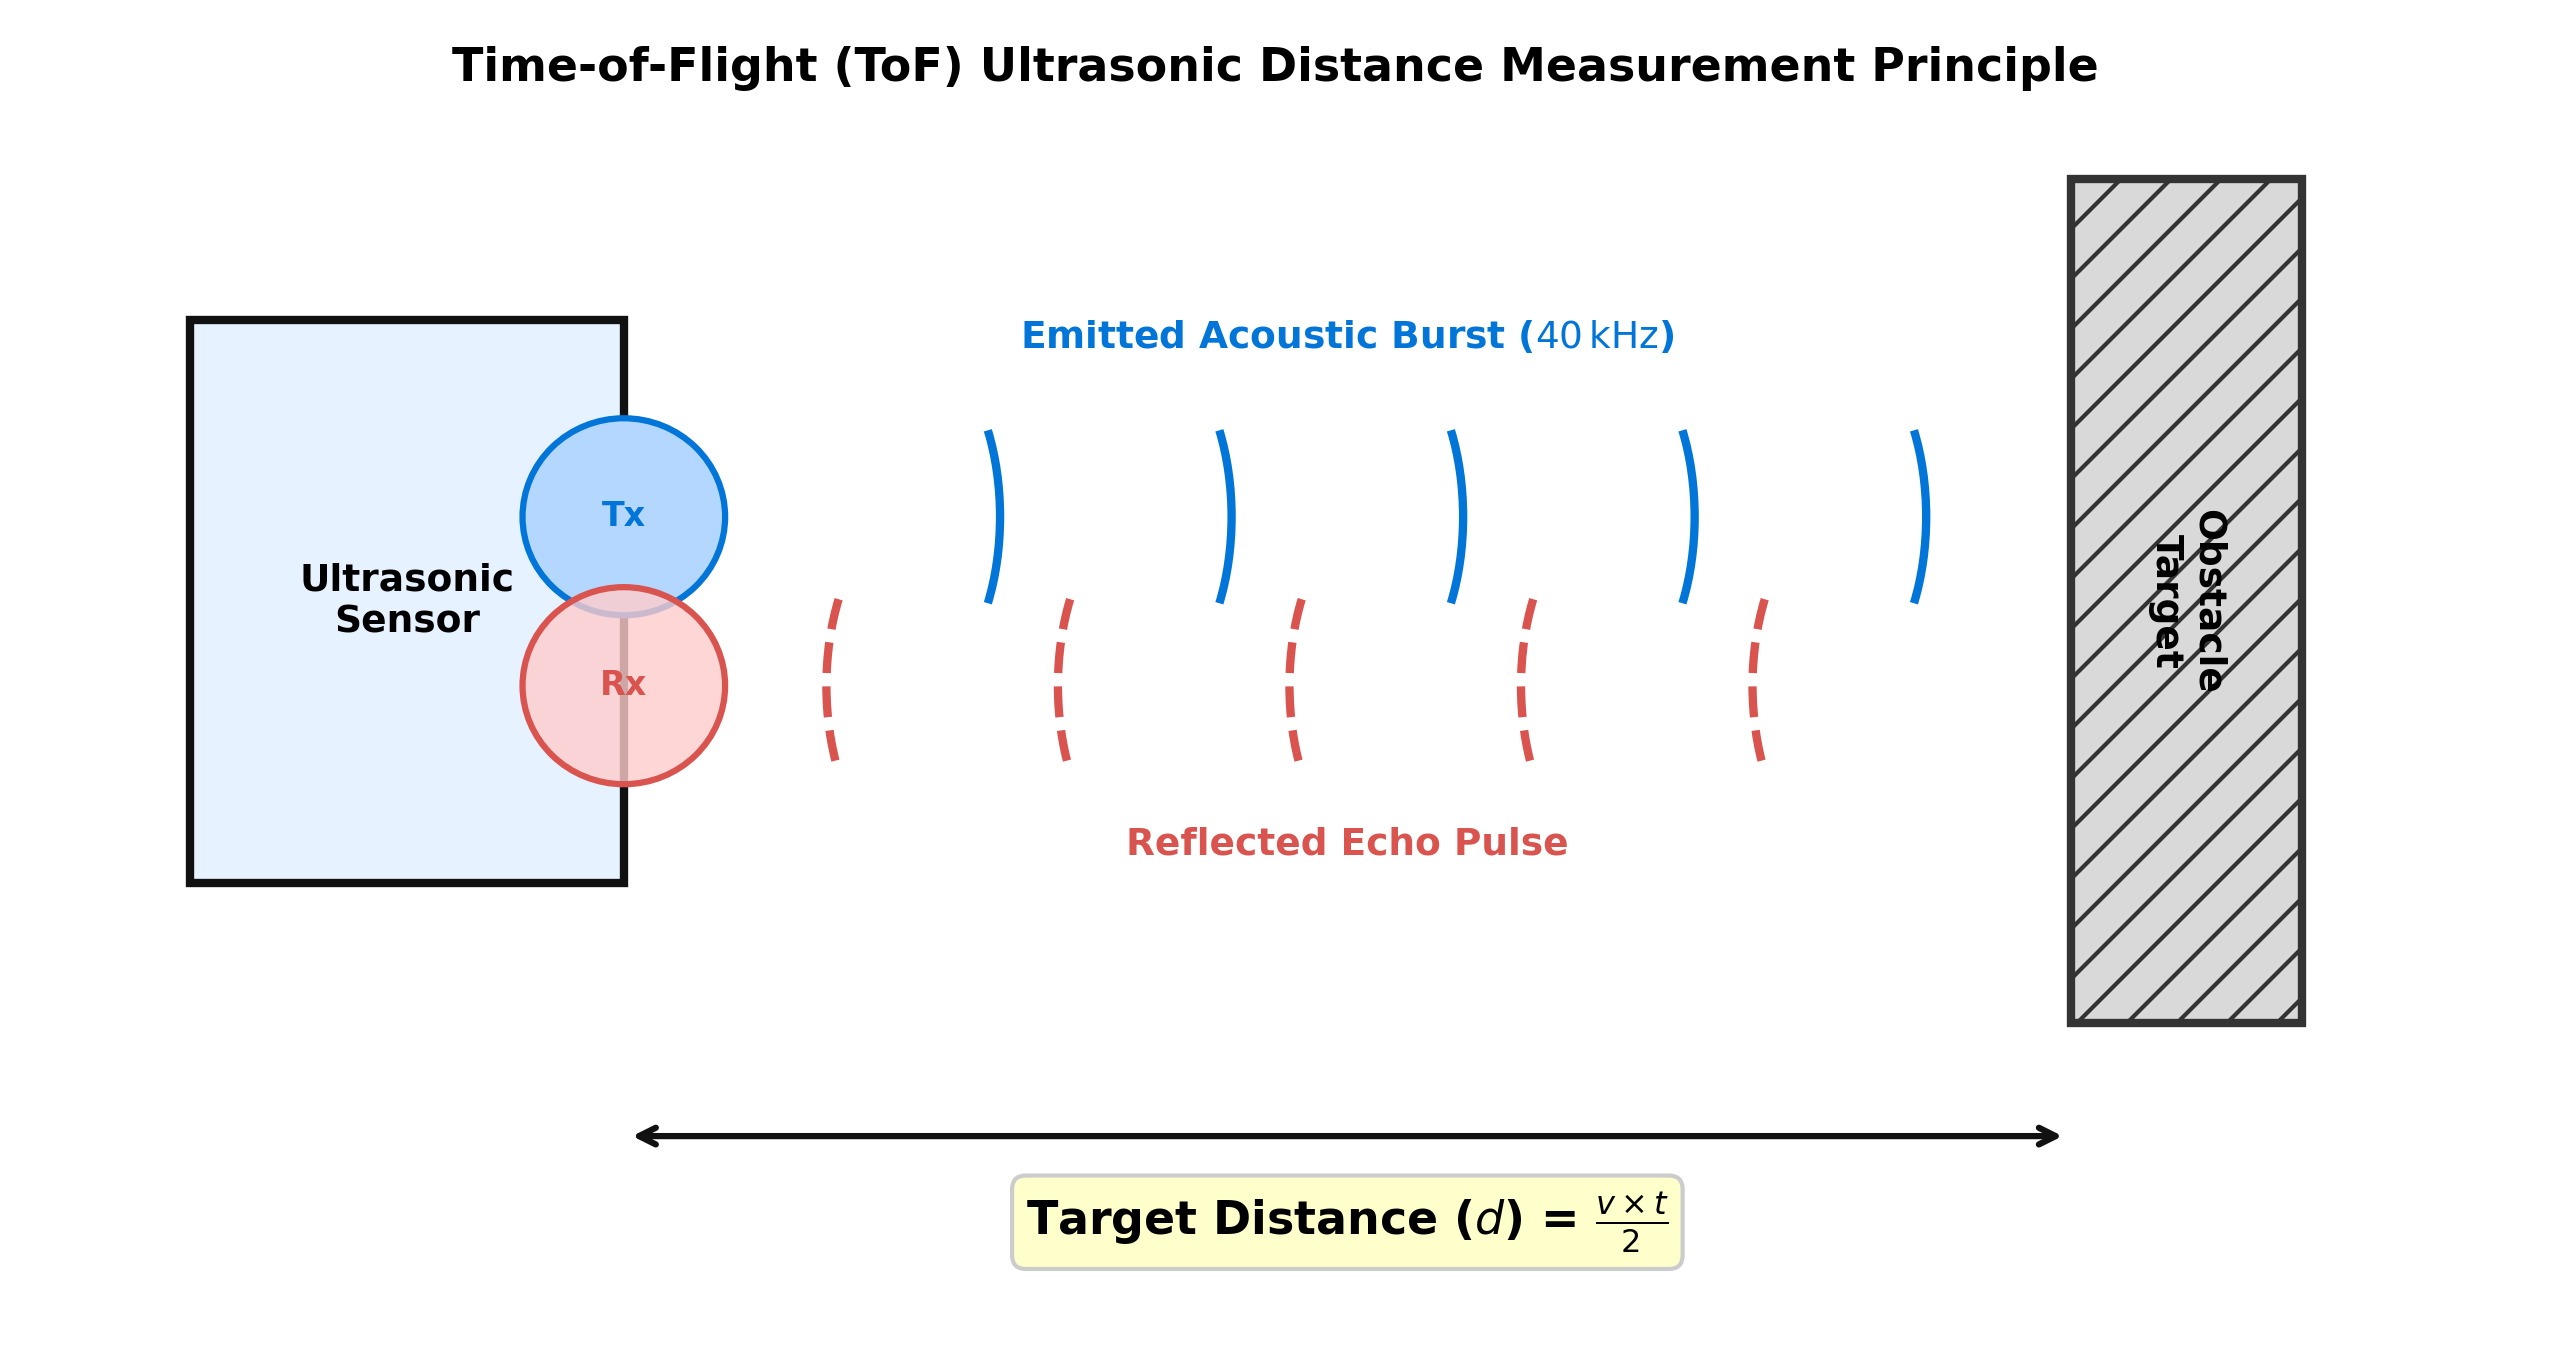
\includegraphics[width=0.80\textwidth]{03_Figures/Ch5/ultrasonic_tof_principle.png}
  \caption{Ultrasonic Time-of-Flight (ToF) obstacle detection and proximity threshold monitoring.}
  \label{fig:ultrasonic_tof_results}
\end{figure}

\FloatBarrier
\subsection{Auto-Rotation Escape Maneuver}
\label{subsec:autorotation_escape_maneuver}

Beyond passive emergency stopping, the obstacle escape logic was tested. Upon encountering a static obstacle within the proximity threshold, the embedded firmware initiated an automated escape maneuver: the wheelchair executed an in-place rotation until the ultrasonic sensors detected a clear path, restoring control to the user. In testing, this obstacle override routine halted motor actuation within the safety perimeter and completed an in-place rotation until clearance was detected, confirming the functional operation of the safety logic independently of user blink inputs.
